\documentclass[letterpaper]{article}
\usepackage{fullpage}
\usepackage{amssymb}
\usepackage{amsfonts}
\usepackage{amsmath}
\usepackage{stmaryrd}
\usepackage{graphicx}
\usepackage{subfigure}
\usepackage{pslatex}   % Good fonts psType 1 or \usepackage{mathptmx}
\usepackage{varioref}  % smart page, figure, table, and equation referencing
\usepackage{algorithm}
\usepackage{algorithmic}
%\usepackage{algorithm2e}
\usepackage{cancel}
\usepackage[small]{caption}
\usepackage{cancel}
\usepackage{tikz} 
\usetikzlibrary{shapes,snakes}
\usepackage{pgf}
\usepackage{listings}

%\usepackage{fancy headings}

  \newcommand{\eqnref}[1]{Eq. (\ref{#1})}                % Eq. (no)
  \newcommand{\figref}[1]{Figure \ref{#1}}                % Figure (no)
  \newcommand{\tblref}[1]{Table \ref{#1}}                % Table (no)
  \newcommand{\secref}[1]{Section \ref{#1}}                % Section (no)
  \newcommand{\incfig}{\centering\includegraphics*}  % Centered 
  \newcommand{\comment}[1]{\COMMENT{ \textcolor{blue}{ #1} }  }

%DG integrals
\newcommand{\pd}[2]{\frac{ \partial #1}{\partial #2}}
\newcommand{\volint}[1]{ \sum_{e \in \mathcal{T}_{h}}\int_{\Omega_k} #1 d\Omega_{e} }  
\newcommand{\surfint}[1]{\sum_{i\in \mathcal{I}_{h}}\int_{\Gamma^{i}} #1 ds}
\newcommand{\bsurfint}[1]{\sum_{b\in \mathcal{B}_{h}}\int_{\Gamma^{b}} #1 ds}
% Operators
\newcommand{\frechd}[2]{ #1'_{\left[ #2 \right]} }%\left( #3\right)} 
\newcommand{\diver}[1]{\nabla \cdot #1}
\newcommand{\abs}[1]{\left \lvert #1 \right \rvert}
\newcommand{\avg}[1]{\left\{ #1 \right\} }
\newcommand{\jump}[1]{\llbracket #1 \rrbracket}
\newcommand{\mat}[1]{\left[ #1 \right]}
\newcommand{\paren}[1]{\left( #1 \right)}
\newcommand{\sparen}[1]{\left[ #1 \right]}
\newcommand{\twonorm}[1]{\parallel #1 \parallel_{2}}
%variables
\newcommand{\hb}[1]{ {\bf #1}_{h} } % \hb for discrete symbol _{h} and bolded for vector in fields
% Fluxes 
\newcommand{\fc}{\vec{{\bf F}}_{c} \paren{\hb{u}}   }
\newcommand{\fv}{\vec{{\bf F}}_{v} \paren{\hb{u},\nabla \hb{u}} }
\newcommand{\fav}{\vec{{\bf F}}_{ad} \paren{ \epsilon,\hb{u},\nabla \hb{u} } }
\newcommand{\ec}{\vec{{\bf E}}_{c} \paren{\hb{u}}   }
\newcommand{\ev}{\vec{{\bf E}}_{v} \paren{\hb{u},\nabla \hb{u}} }
\newcommand{\eav}{\vec{{\bf E}}_{ad} \paren{ \epsilon,\hb{u},\nabla \hb{u} } }

\newcommand{\hc}{\mathcal{H}_{c} \paren{ \hb{u}^{+},\hb{u}^{-},\vec{n} } }  
\newcommand{\hv}{\mathcal{H}_{v} \paren{ \hb{u},\hb{u}^{-},\phi_{i}^{+}, \phi_{i}^{-},\nabla \hb{u}^{+},\nabla \hb{u}^{-},
\vec{n} } }
\newcommand{\hav}{\mathcal{H}_{ad}\paren{ \epsilon^{+},\epsilon^{-},\hb{u}^{+},\hb{w}^{+}, \hb{w}^{-},\hb{u}^{-},\nabla \hb{u}^{+},\nabla \hb{u}^{-},\vec{n} } }
\newcommand{\hcb}{\mathcal{H}_{c}^{b} \paren{ \hb{u}^{b} \paren{ \hb{u}^{+} },\vec{n} } } 
\newcommand{\hvb}{\mathcal{H}_{v}^{b} \paren{ \hb{u}^{b} \paren{\hb{u}^{+}},\phi_{i}^{+},\nabla \hb{u}^{+},\vec{n} } }
\newcommand{\havb}{\mathcal{H}_{ad}^{b} \paren{ \epsilon^{+}, \hb{u}^{b}\paren{ \hb{u}^{+}},{\bf w}^{+}, \nabla \hb{u}^{+},\vec{n} } }
%Non-linear variables
\newcommand{\Resid}[1] {{\bf R}(#1)}
\newcommand{\Residp}[1] {{\bf R}_{p}(#1)}
%FIgures
\newcommand{\figwidth}{.48\textwidth}
\newcommand{\lfigwidth}{.68\textwidth} %small version .68, large version .75
%%% Footer
%\lfoot[\fancyplain{}{}]{Approved for public release \\ distribution unlimited.}
\newcommand{\createav}{CREATE\textsuperscript{TM}-AV }

%%%%% Listings environments
\lstdefinestyle{Meshfile}
{
sensitive=false,
keywordstyle=\color{blue},
morekeywords={Nodes, Elements, BcFaces, BcID, Connectivity, Nodal, Boundary, Face, IDs},
basicstyle=\ttfamily,
numbers=left, 
numberstyle=\ttfamily\color{gray}\small, 
numbersep=5pt, 
frame=single, 
rulecolor=\color{black}, 
framexrightmargin=5pt,
backgroundcolor=\color{white}, 
}


\title{Unstructured Meshes}
\author{Nicholas K. Burgess}
\begin{document}
\maketitle
\section{Introduction}
Unstructured mesh connectivity is the critical component of developing an unstructured mesh PDE solver.  In the case of structured meshes, where connectivity is implicit, the neighbors of a point or element are increments of $\pm 1$ to the dimension indicies.  Conversely, unstructured meshes store connectivity explicitly in certain helpful data structures.  Unfortunately, unstructured mesh generators do not provide all the connectivity required to make a useful PDE solver.  Therefore, using the connectivity provided by the mesh generator so-called auxiliary or extra connectivity must be constructed.  

The construction of auxiliary connectivity can be considered a subject unto itself and many individuals devote large amounts of their development time towards building newer and more helpful connectivity structures.  The exact algorithms for constructing auxiliary connectivity are beyond the scope of this document.  However, this document will explain a subset of necessary auxiliary connectivity required for finite-volume methods on unstructured meshes.    

\section{Mesh Connectivity}
Unstructured mesh generators are normally stand-alone programs that take in geometry and build a mesh of that geometry.  One normally interacts with the mesh produced by the generator using a file.  Some advanced applications interact with mesh generators through application programming  interfaces or (APIs), it is assumed this is not the case for the purposed of this demonstration.  

Assuming one obtains a valid mesh file from a mesh generator one can expect to find the following data in this file.  
\begin{lstlisting}[style=Meshfile]
Nodes "Number of nodes in the mesh"
Elements "Number of elements in the mesh
BcFaces "Number of boundary faces in the mesh"
BcID "Number of boundary ID numbers of boundaries"
Nodal Coordinates
x0 y0 z0 
x1 y1 z1 
x2 y2 z2 
x3 y3 z3
.     .    .
xNodes yNodes zNodes
Element to Node Connectivity
Element1 Node1 Node2 Node3 Node4 ... NodeN
Element2 Node1 Node2 Node3 Node4 ... NodeN
Element3 Node1 Node2 Node3 Node4 ... NodeN
.     .    .    .     .    ...     .
ElementE Node1 Node2 Node3 Node4 ... NodeN
Boundary Face to Node Connecitivity
Face1 Node1 Node2 ... NodeN
Face2 Node1 Node2 ... NodeN
.     .      .   ...      .
FaceBF Node1 Node2 ... NodeN
Boundary IDs for each boundary face
Face1 ID1
Face2 ID2
.
FaceBF ID2
\end{lstlisting}
The mesh file provides only some of the connectivity required for PDE solvers.  The following tables describe the various connectivity formed and used by unstructured finite-volume based PDE solvers.  
\subsection{Definition of Nodes}
The most fundamental quantity of an unstructured mesh is a node.  A node is an entity whose only attribute is coordinates $\vec{x} \in \mathbb{R}^{d}$.  Nodal coordinates are simply tabulated as in the notional mesh file.  
\subsection{Definition of Elements}
Elements are collections of nodes that form canonical shapes.  The listing of which nodes make up which elements is known as element to node connectivity.  The faces that make up an element are tracked by element to face connectivity, which indicates which faces make up an element.  One also connects elements to elements, which is also known as element adjacency, via the element to element connectivity.      

The  canonical element shapes are detailed in the following sections.  Each section displays figures detailing the nodes, edges, and faces making up each canonical shape.  
\begin{figure}[h!]
\centering
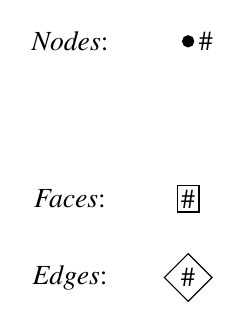
\begin{tikzpicture}[inner sep=.5mm,minimum size=.5mm]
\node at (.5, 0.0) [circle,draw=black,fill=black] (Node1) {};
\node at (Node1.east)[black,right] (a0) {$\#$} ;
\node at (.5,-2.0) [rectangle,draw=black] (elem2){$\#$};
\node at (.5,-3.0) [diamond,draw=black] (elem3){$\#$};
\node at(-1.0,0.0) (nameN) {\textit{Nodes}:} ;
\node at(-1.0,-2.0) (nameF) {\textit{Faces}:} ;
\node at(-1.0,-3.0) (nameF) {\textit{Edges}:} ;
\end{tikzpicture}
\caption{Numbering symbols used to denote, nodes, faces and edges of canonical elements.}
\end{figure}
          
 \subsubsection{1-D Bar}
In one spatial dimension only one type of element is available.  This element in known as the ``bar'' element.  The ``bar'' element (shown in \figref{fig:c3_line}) is constructed by taking two nodes of the mesh and connecting them by a line segment.  
\begin{figure}[h!]
\centering
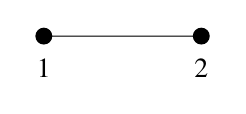
\begin{tikzpicture}
\draw[fill = black]  (0,0) circle (.1cm) -- (2,0) circle(.1cm) ;
\draw (0,-.4) node {1} (2,-.4) node {2};
\end{tikzpicture}
\caption{1-D ``bar'' element.}
\label{fig:c3_line}
\end{figure}

\subsubsection{2-D Triangle}
In two spatial dimensions there are two element types available one of which is the triangle.  The triangle is defined by connecting 3 of the mesh nodes as in \figref{fig:c3_triangle}.  Note that faces and edges are the same in 2-D.  
\begin{figure}[h!]
\centering
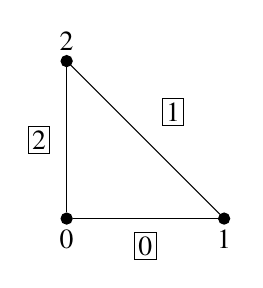
\begin{tikzpicture}[inner sep=.5mm,minimum size=.5mm]
\node at (0,0) [circle,draw=black,fill=black] (Node1) {};
\node at (2,0) [circle,draw=black,fill=black] (Node2) {};
\node at (0,2) [circle,draw=black,fill=black] (Node3) {};
\node [black,below] at (Node1.south) {0};
\node [black,below] at (Node2.south) {1};
\node [black,above] at (Node3.north) {2};
\draw (Node1) -- (Node2);
\draw (Node2) -- (Node3);
\draw (Node3) -- (Node1);
\node at (1,-.35) [rectangle,draw=black] {0};
\node at (1.35,1.35) [rectangle,draw=black] {1};
\node at (-.35,1.0) [rectangle,draw=black] {2};

\end{tikzpicture}
\caption{2-D Triangle Element.}
\label{fig:c3_triangle}
\end{figure}
\subsubsection{2-D Quadrilateral}
The other element type in two spatial dimension is the quadrilateral, which is defined by connecting 4 nodes of the mesh as shown in \figref{fig:c3_quad}.  Note that faces and edges are the same in 2-D.  
\begin{figure}[h!]
\centering
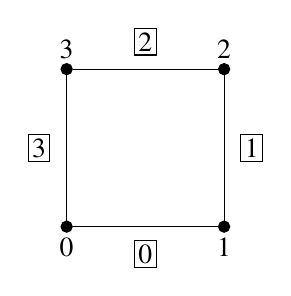
\begin{tikzpicture}[inner sep=.5mm,minimum size=.5mm]
\node at (0,0) [circle,draw=black,fill=black] (Node1) {};
\node at (2,0) [circle,draw=black,fill=black] (Node2) {};
\node at (2,2) [circle,draw=black,fill=black] (Node3) {};
\node at (0,2) [circle,draw=black,fill=black] (Node4) {};
\node [black,below] at (Node1.south) {0};
\node [black,below] at (Node2.south) {1};
\node [black,above] at (Node3.north) {2};
\node [black,above] at (Node4.north) {3};
\draw (Node1) -- (Node2);
\draw (Node2) -- (Node3);
\draw (Node3) -- (Node4);
\draw (Node4) -- (Node1);
\node at (1,-.35) [rectangle,draw=black] {0};
\node at (2.35,1) [rectangle,draw=black] {1};
\node at (1.0,2.35) [rectangle,draw=black] {2};
\node at (-.35, 1.0)  [rectangle,draw=black] {3};
\end{tikzpicture}
\caption{2-D Triangle Element.}
\label{fig:c3_quad}
\end{figure}
\subsubsection{3-D Tetrahedra}
Tetrahedral elements contain four nodes, four triangular faces and six edges.  \figref{fig:c3_3D_tet_elem} and \figref{fig:c3_3D_tet_edge} show the definitions of the tetrahedra nodes, edges, and faces.  
\begin{figure}[h!]
\centering
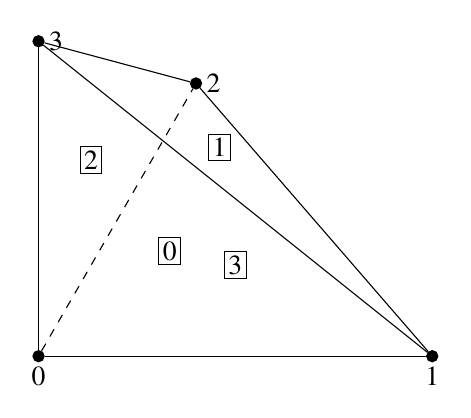
\begin{tikzpicture}[inner sep=.5mm,minimum size=.5mm]
%Node Coordinates
\node at (-2,-2) [circle,draw=black,fill=black] (Node1) {};
\node at (3,-2) [circle,draw=black,fill=black] (Node2) {};
\node at (0.0, 1.464) [circle,draw=black,fill=black] (Node3) {};
\node at (-2, 2) [circle,draw=black,fill=black] (Node4) {};
%Node Labels
\node [black,below] at (Node1.south) {0};
\node [black,below] at (Node2.south) {1};
\node [black,right] at (Node3.east) {2};
\node [black,right] at (Node4.east){3};
%Connections
\draw (Node1) -- (Node2);
\draw [dashed] (Node1) -- (Node3);
\draw (Node1) -- (Node4);
\draw (Node2) -- (Node3);
\draw (Node2) -- (Node4);
\draw (Node3) -- (Node4);
% Element Labels
\node at (-.33333,-.6666667)  [rectangle,draw=black] {0};
\node at (.3,.65)  [rectangle,draw=black] {1};
\node at (-1.3333, .488803)  [rectangle,draw=black] {2};
\node at (.5, -.845299)  [rectangle,draw=black] {3};

\end{tikzpicture}
\caption{Tetrahedral Element, $\vec{x} \in [-1,1]^{3}$.}
\label{fig:c3_3D_tet_elem}
\end{figure}

\begin{figure}[h!]
\centering
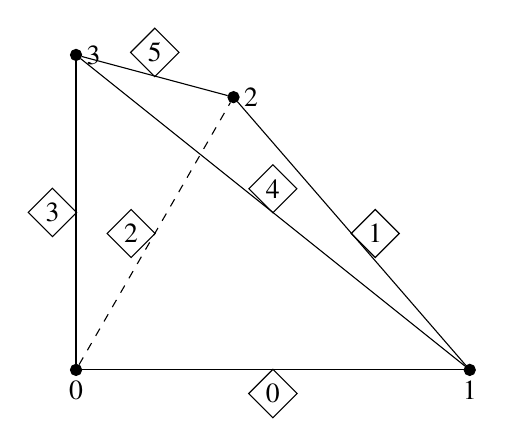
\begin{tikzpicture}[inner sep=.5mm,minimum size=.5mm]
%Node Coordinates
\node at (-2,-2) [circle,draw=black,fill=black] (Node1) {};
\node at (3,-2) [circle,draw=black,fill=black] (Node2) {};
\node at (0.0, 1.464) [circle,draw=black,fill=black] (Node3) {};
\node at (-2, 2) [circle,draw=black,fill=black] (Node4) {};
%Node Labels
\node [black,below] at (Node1.south) {0};
\node [black,below] at (Node2.south) {1};
\node [black,right] at (Node3.east) {2};
\node [black,right] at (Node4.east){3};
%Connections
\draw (Node1) -- (Node2);
\draw [dashed] (Node1) -- (Node3);
\draw (Node1) -- (Node4);
\draw (Node2) -- (Node3);
\draw (Node2) -- (Node4);
\draw (Node3) -- (Node4);
% Edge labels
\node at (.5,-2.3)  [diamond,draw=black] {0};
\node at (1.8,-.267949)  [diamond,draw=black] {1};
\node at (-1.3, -.267949)  [diamond,draw=black] {2};
\node at (-2.3, 0.0)  [diamond,draw=black] {3};
\node at (.5, .3) [diamond,draw=black] {4};
\node at (-1.0, 2.032051) [diamond,draw=black] {5};
\end{tikzpicture}
\caption{Tetrahedral Element edges, $\vec{x} \in [-1,1]^{3}$.}
\label{fig:c3_3D_tet_edge}
\end{figure}

\subsubsection{3-D Prism}
Prismatic elements contain six nodes, 2 triangular faces, 3 quadrilateral faces, and nine edges.  \figref{fig:c3_3D_prism_elem} and \figref{fig:c3_3D_prism_edge} show the definitions of the prism nodes, edges, and faces.  
\begin{figure}[h!]
\centering
\begin{tikzpicture}[inner sep=.5mm,minimum size=.5mm]
%Node Coordinates
\node at (-2,-2) [circle,draw=black,fill=black] (Node1) {};
\node at (3,-2) [circle,draw=black,fill=black] (Node2) {};
\node at (0.0,1.464) [circle,draw=black,fill=black] (Node3) {};
\node at (-2, 2) [circle,draw=black,fill=black] (Node4) {};
\node at (3, 2) [circle,draw=black,fill=black] (Node5) {};
\node at (0, 5.464) [circle,draw=black,fill=black] (Node6) {};

%Node Labels
\node [black,below] at (Node1.south) {0};
\node [black,below] at (Node2.south) {1};
\node [black,right] at (Node3.east) {2};
\node [black,left] at (Node4.west){3};
\node [black,right] at (Node5.east) {4};
\node [black,above] at (Node6.north){5};
%Connections
\draw (Node1) -- (Node2);
\draw [dashed] (Node2) -- (Node3);
\draw [dashed] (Node3) -- (Node1);
\draw (Node4) -- (Node5);
\draw (Node5) -- (Node6);
\draw (Node6) -- (Node4);
\draw (Node1) -- (Node4);
\draw (Node2) -- (Node5);
\draw [dashed] (Node3) -- (Node6);
%Face Labels
\node at (.5,0.0)  [rectangle,draw=black] {0};
\node at (1.5, 1.73205)  [rectangle,draw=black] {1};
\node at (-1.0,  1.73205)  [rectangle,draw=black] {2};
\node at (.3333333, -.845299) [rectangle,draw=black] {3};
\node at (.3333333, 3.154700) [rectangle,draw=black] {4};
\end{tikzpicture}
\caption{Prismatic Element, $\vec{x} \in [-1,1]^{3}$.}
\label{fig:c3_3D_prism_elem}
\end{figure}

\begin{figure}[h!]
\centering
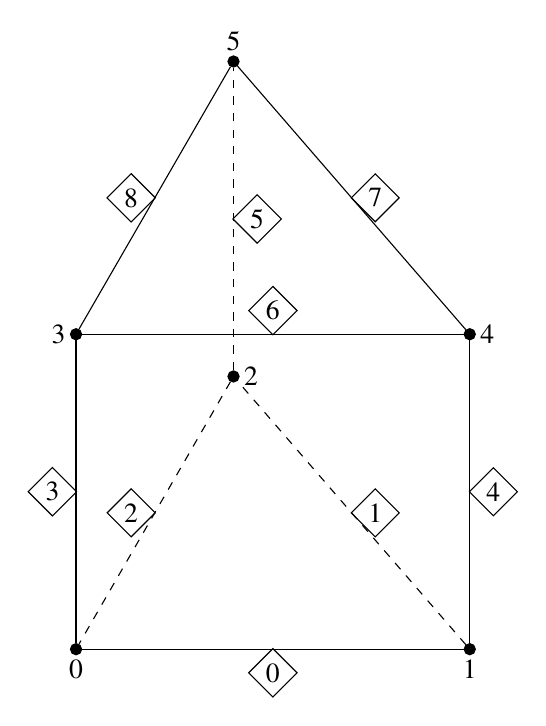
\begin{tikzpicture}[inner sep=.5mm,minimum size=.5mm]
%Node Coordinates
\node at (-2,-2) [circle,draw=black,fill=black] (Node1) {};
\node at (3,-2) [circle,draw=black,fill=black] (Node2) {};
\node at (0.0,1.464) [circle,draw=black,fill=black] (Node3) {};
\node at (-2, 2) [circle,draw=black,fill=black] (Node4) {};
\node at (3, 2) [circle,draw=black,fill=black] (Node5) {};
\node at (0, 5.464) [circle,draw=black,fill=black] (Node6) {};

%Node Labels
\node [black,below] at (Node1.south) {0};
\node [black,below] at (Node2.south) {1};
\node [black,right] at (Node3.east) {2};
\node [black,left] at (Node4.west){3};
\node [black,right] at (Node5.east) {4};
\node [black,above] at (Node6.north){5};
%Connections
\draw (Node1) -- (Node2);
\draw [dashed] (Node2) -- (Node3);
\draw [dashed] (Node3) -- (Node1);
\draw (Node4) -- (Node5);
\draw (Node5) -- (Node6);
\draw (Node6) -- (Node4);
\draw (Node1) -- (Node4);
\draw (Node2) -- (Node5);
\draw [dashed] (Node3) -- (Node6);
% Edge Labels
\node at (.5, -2.3) [diamond, draw=black]{0};
\node at (1.8, -.267949) [diamond, draw=black]{1};
\node at (-1.3, -.267949) [diamond, draw=black]{2};
\node at (-2.3, 0.0) [diamond, draw=black]{3};
\node at (3.3, 0.0) [diamond, draw=black]{4};
\node at (.3, 3.4641016) [diamond, draw=black]{5};
\node at (.5, 2.3) [diamond, draw=black]{6};
\node at (1.8, 3.7320) [diamond, draw=black]{7};
\node at (-1.3, 3.7320) [diamond, draw=black]{8};
\end{tikzpicture}
\caption{Prismatic Element edges, $\vec{x} \in [-1,1]^{3}$.}
\label{fig:c3_3D_prism_edge}
\end{figure}

\subsubsection{3-D Pyramid}
Pyramid elements are comprised of fives nodes, 4 triangular faces, 1 quadrilateral face, and eight edges.  \figref{fig:c3_3D_pyramid_elem} and \figref{fig:c3_3D_pyramid_edge} show the definition of the prism nodes, edges, and faces.  
\begin{figure}[h!]
\centering
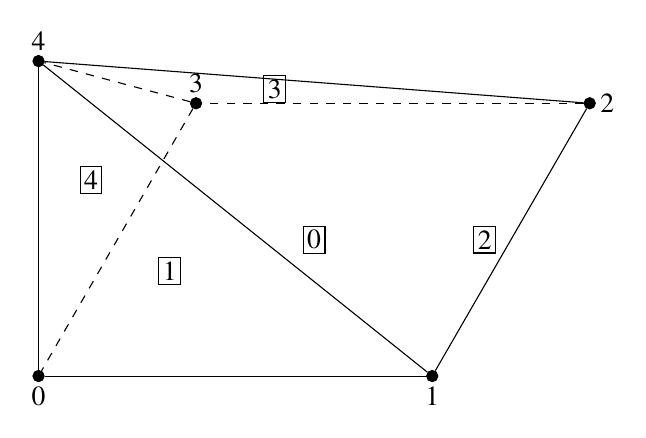
\begin{tikzpicture}[inner sep=.5mm,minimum size=.5mm]
%Node Coordinates
\node at (-2,-2) [circle,draw=black,fill=black] (Node1) {};
\node at (3,-2) [circle,draw=black,fill=black] (Node2) {};
\node at (5, 1.46410) [circle,draw=black,fill=black] (Node3) {};
\node at (0.0, 1.46410) [circle,draw=black,fill=black] (Node4) {};
\node at (-2, 2) [circle,draw=black,fill=black] (Node5) {};
%Node Labels
\node [black,below] at (Node1.south) {0};
\node [black,below] at (Node2.south) {1};
\node [black,right] at (Node3.east) {2};
\node [black,above] at (Node4.north){3};
\node [black,above] at (Node5.north) {4};
%connections
\draw (Node1) -- (Node2);
\draw (Node2) -- (Node3);
\draw [dashed] (Node3) -- (Node4);
\draw [dashed] (Node4) -- (Node1);
\draw (Node1) -- (Node5);
\draw (Node2) -- (Node5);
\draw (Node3) -- (Node5);
\draw [dashed] (Node4) -- (Node5);
%Face Labels
\node at (1.5,-.267949)  [rectangle,draw=black] {0};
\node at (-.33333, -.666667)  [rectangle,draw=black] {1};
\node at (3.666667, -.267949)  [rectangle,draw=black] {2};
\node at (1.00, 1.64273) [rectangle,draw=black] {3};
\node at (-1.3333333, .4880338) [rectangle,draw=black] {4};
\end{tikzpicture}
\caption{Pyramid Element, $\vec{x} \in [-1,1]^{3}$.}
\label{fig:c3_3D_pyramid_elem}
\end{figure}

\begin{figure}[h!]
\centering
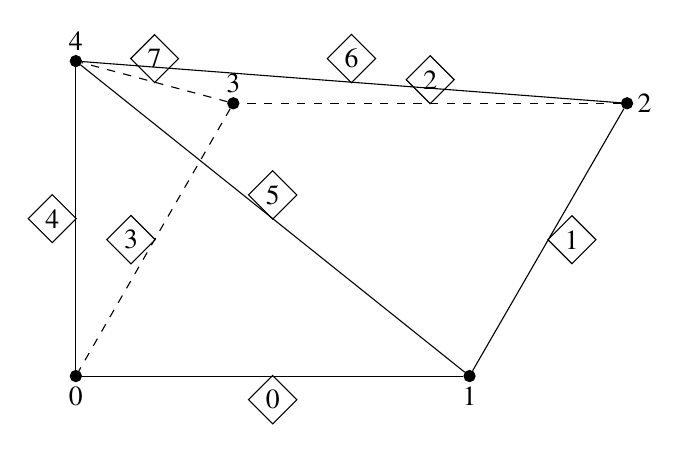
\begin{tikzpicture}[inner sep=.5mm,minimum size=.5mm]
%Node Coordinates
\node at (-2,-2) [circle,draw=black,fill=black] (Node1) {};
\node at (3,-2) [circle,draw=black,fill=black] (Node2) {};
\node at (5, 1.46410) [circle,draw=black,fill=black] (Node3) {};
\node at (0.0, 1.46410) [circle,draw=black,fill=black] (Node4) {};
\node at (-2, 2) [circle,draw=black,fill=black] (Node5) {};
%Node Labels
\node [black,below] at (Node1.south) {0};
\node [black,below] at (Node2.south) {1};
\node [black,right] at (Node3.east) {2};
\node [black,above] at (Node4.north){3};
\node [black,above] at (Node5.north) {4};
%connections
\draw (Node1) -- (Node2);
\draw (Node2) -- (Node3);
\draw [dashed] (Node3) -- (Node4);
\draw [dashed] (Node4) -- (Node1);
\draw (Node1) -- (Node5);
\draw (Node2) -- (Node5);
\draw (Node3) -- (Node5);
\draw [dashed] (Node4) -- (Node5);
% Edges
\node at (.5, -2.3) [diamond, draw=black]{0};
\node at (4.3, -.267949) [diamond, draw=black]{1};
\node at (2.5, 1.7641016) [diamond, draw=black]{2};
\node at (-1.3,-.267949) [diamond, draw=black]{3};
\node at (-2.3, 0.0) [diamond, draw=black]{4};
\node at (.5, 0.3) [diamond, draw=black]{5};
\node at (1.5, 2.03205) [diamond, draw=black]{6};
\node at (-1.0, 2.03205) [diamond, draw=black]{7};

\end{tikzpicture}
\caption{Pyramid Element Edges, $\vec{x} \in [-1,1]^{3}$.}
\label{fig:c3_3D_pyramid_edge}
\end{figure}


\subsubsection{3-D Hexahedra}
Hexahedral elements are comprised of eight nodes, six quadrilateral faces, and twelve edges.  \figref{fig:c3_3D_hex_elem} and \figref{fig:c3_3D_hex_edge} show the definition of the prism nodes, edges, and faces.   
\begin{figure}[h!]
\centering
\begin{tikzpicture}[inner sep=.5mm,minimum size=.5mm]
\node at (-2,-2) [circle,draw=black,fill=black] (Node1) {};
\node at (3,-2) [circle,draw=black,fill=black] (Node2) {};
\node at (5, 1.46410) [circle,draw=black,fill=black] (Node3) {};
\node at (0.0, 1.46410) [circle,draw=black,fill=black] (Node4) {};
\node at (-2, 2) [circle,draw=black,fill=black] (Node5) {};
\node at (3, 2) [circle,draw=black,fill=black] (Node6) {};
\node at (5, 5.4641016) [circle,draw=black,fill=black] (Node7) {};
\node at (0.0, 5.46410) [circle,draw=black,fill=black] (Node8) {};
% Node Labels
\node [black,below] at (Node1.south) {0};
\node [black,below] at (Node2.south) {1};
\node [black,right] at (Node3.east) {2};
\node [black,left] at (Node4.west){3};
\node [black,left] at (Node5.west) {4};
\node [black,right] at (Node6.east) {5};
\node [black,right] at (Node7.east) {6};
\node [black,above] at (Node8.north) {7};
% Node Connections
\draw (Node1) -- (Node2);
\draw (Node2) -- (Node3);
\draw [dashed] (Node3) -- (Node4);
\draw [dashed] (Node4) -- (Node1);
\draw (Node1) -- (Node5);
\draw (Node2) -- (Node6);
\draw (Node3) -- (Node7);
\draw [dashed] (Node4) -- (Node8);
\draw (Node5) -- (Node6);
\draw (Node6) -- (Node7);
\draw (Node7) -- (Node8);
\draw (Node8) -- (Node5);
% Face Labels
\node at (-1.0,1.73205)  [rectangle,draw=black] {0};
\node at (4.0, 1.73205)  [rectangle,draw=black] {1};
\node at (.5, 0.0)  [rectangle,draw=black] {2};
\node at (2.5, 3.4641016) [rectangle,draw=black] {3};
\node at (1.5, -.267949) [rectangle,draw=black] {4};
\node at (1.5, 3.73205) [rectangle,draw=black] {5};
\end{tikzpicture}
\caption{Hexhedral Element, $\vec{x} \in [-1,1]^{3}$.}
\label{fig:c3_3D_hex_elem}
\end{figure}

\begin{figure}[h!]
\centering
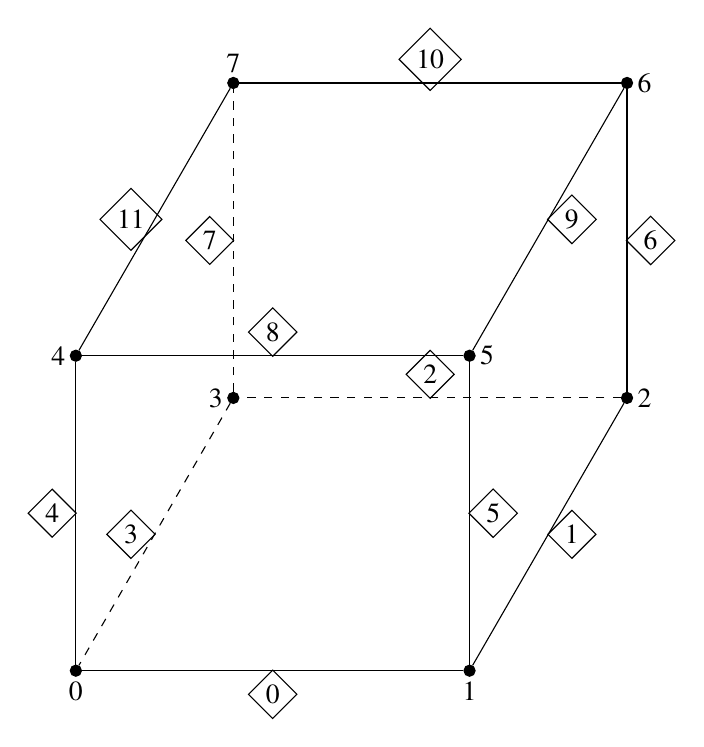
\begin{tikzpicture}[inner sep=.5mm,minimum size=.5mm]
\node at (-2,-2) [circle,draw=black,fill=black] (Node1) {};
\node at (3,-2) [circle,draw=black,fill=black] (Node2) {};
\node at (5, 1.46410) [circle,draw=black,fill=black] (Node3) {};
\node at (0.0, 1.46410) [circle,draw=black,fill=black] (Node4) {};
\node at (-2, 2) [circle,draw=black,fill=black] (Node5) {};
\node at (3, 2) [circle,draw=black,fill=black] (Node6) {};
\node at (5, 5.4641016) [circle,draw=black,fill=black] (Node7) {};
\node at (0.0, 5.46410) [circle,draw=black,fill=black] (Node8) {};
% Node Labels
\node [black,below] at (Node1.south) {0};
\node [black,below] at (Node2.south) {1};
\node [black,right] at (Node3.east) {2};
\node [black,left] at (Node4.west){3};
\node [black,left] at (Node5.west) {4};
\node [black,right] at (Node6.east) {5};
\node [black,right] at (Node7.east) {6};
\node [black,above] at (Node8.north) {7};
% Node Connections
\draw (Node1) -- (Node2);
\draw (Node2) -- (Node3);
\draw [dashed] (Node3) -- (Node4);
\draw [dashed] (Node4) -- (Node1);
\draw (Node1) -- (Node5);
\draw (Node2) -- (Node6);
\draw (Node3) -- (Node7);
\draw [dashed] (Node4) -- (Node8);
\draw (Node5) -- (Node6);
\draw (Node6) -- (Node7);
\draw (Node7) -- (Node8);
\draw (Node8) -- (Node5);
% Edge Labels
\node at (.5, -2.3) [diamond, draw=black]{0};
\node at (4.3, -.267949) [diamond, draw=black]{1};
\node at (2.5, 1.7641016) [diamond, draw=black]{2};
\node at (-1.3,-.267949) [diamond, draw=black]{3};
\node at (-2.3, 0.0) [diamond, draw=black]{4};
\node at (3.3, 0.0) [diamond, draw=black]{5};
\node at (5.3, 3.46410) [diamond, draw=black]{6};
\node at (-.3, 3.4641016) [diamond, draw=black]{7};
\node at (.5, 2.3) [diamond, draw=black]{8};
\node at (4.3, 3.73205) [diamond, draw=black]{9};
\node at (2.5, 5.7641016) [diamond, draw=black]{10};
\node at (-1.3,3.73205) [diamond, draw=black]{11};

\end{tikzpicture}
\caption{Hexhedral Element edges, $\vec{x} \in [-1,1]^{3}$.}
\label{fig:c3_3D_hex_edge}
\end{figure}

 \subsection{Definition of Interior Faces}
 Interior faces are mesh entities that connect two elements (volumes).  Examining the notional mesh file indicates that the mesh generator does not provide interior face definitions.  A face is made up of nodes and has the property of a signed area vector ($i.e.$ a normal whose magnitude is the face area).  \figref{fig:face_def} gives the definition of a face as connecting two elements.  Note that a face has a unique normal vector that points out of one element and into another.  The element from which the normal vector points in denoted the "left" element and the element into which the normal points is denoted the "right" element.  Note that the terms "left" and "right" are used only as jargon here and do not denote any information about actual relative position in space.  
 \begin{figure}[h!]
\centering
\includegraphics[width=\lfigwidth]{face_def.pdf}
\caption{Definition of a face in an unstructured tetrahedral mesh.}
\label{fig:face_def}
\end{figure}

Faces also have canonical shapes.  In one spatial dimension a face is a node, two spatial dimension an edge, and three spatial dimensions triangles or quadrilaterals.  Similarly to elements, faces are made up of nodes and a face to node connectivity is normally formed.    
\subsection{Boundary Face to Element}
While interior faces connect two elements together, boundary faces connect elements to what is beyond the computational domain.  \figref{fig:bc_face_def} gives an example of a boundary face.  Similarly to interior faces boundary faces have a normal vector.  
 \begin{figure}[h!]
\centering
\includegraphics[width=\figwidth]{bc_face_def.pdf}
\caption{Definition of a boundary face in an unstructured tetrahedral mesh.}
\label{fig:bc_face_def}
\end{figure}

By convention the boundary normal vector points out of the domain or away from the element connected to the boundary face.  The element to connected to each boundary face is an important connectivity that is explicitly tracked by a PDE solver.   Boundary faces are also comprised of nodes with a boundary face to node connectivity have the same and have the same canonical shapes as interior faces.  

In order to keep track of what boundary conditions are be applied to each boundary face, a boundary ID connectivity is usually stored.  This connectivity is simply an integer specifying and ID number for each boundary face.  Boundary conditions are applied uniquely to each boundary ID, and all boundary faces having the same ID number have the same boundary condition.    

\section{Unstructured Mesh Cheat Sheet}
\subsection{Element Connectivity}
This section gives notional tables for defining elements.  
\begin{table}[h!]
\centering
\begin{tabular}{|ccccc|}
\hline
Element \#  & $1^{st}$ Node  & Second Node & \dots & $N^{th}$ Node \\
\hline
 0 & $Node_{0}$ & $Node_{1}$ & \dots & $Node_{N-1}$ \\
 1 & $Node_{0}$ & $Node_{1}$ & \dots & $Node_{N-1}$ \\
  \vdots & \vdots & \vdots & \vdots & \vdots \\
  $N_{elements}$ & $Node_{0}$ & $Node_{1}$ & \dots & $Node_{N-1}$ \\
\hline 
\end{tabular}
\caption{Element to node connectivity.}
\end{table}

\begin{table}[h!]
\centering
\begin{tabular}{|c|cccc|}
\hline
Element \#  & $1^{st}$ Face  & Second Face & \dots & $N^{th}$ Face \\
\hline
 0 & $Face_{0}$ & $Face_{1}$ & \dots & $Face_{N-1}$ \\
 1 & $Face_{0}$ & $Face_{1}$ & \dots & $Face_{N-1}$ \\
  \vdots & \vdots & \vdots & \vdots & \vdots \\
  $N_{elements}$ & $Face_{0}$ & $Face_{1}$ & \dots & $Face_{N-1}$ \\
\hline 
\end{tabular}
\caption{Element to face connectivity.  NOTE: Boundary faces are usually denoted with a negative value of magnitude one higher than the actual number. }
\end{table}

\begin{table}[h!]
\centering
\begin{tabular}{|c|cccc|}
\hline
Element \#  & $1^{st}$ Element  & Second Element & \dots & $N^{th}$ Element \\
\hline
 0 & $Element_{0}$ & $Element_{1}$ & \dots & $Element_{N-1}$ \\
 1 & $Element_{0}$ & $Element_{1}$ & \dots & $Element_{N-1}$ \\
  \vdots & \vdots & \vdots & \vdots & \vdots \\
  $N_{elements}$ & $Element_{0}$ & $Element_{1}$ & \dots & $Element_{N-1}$ \\
\hline 
\end{tabular}
\caption{Element to element connectivity or more formally known as element adjacency.  NOTE: Element adjacency includes element self adjacency. }
\end{table}

\subsection{Face Connectivity}
This section gives notional tables defining connectivity for faces.  
\begin{table}[h!]
\centering
\begin{tabular}{|c|cccc|}
\hline
Face \#  & $1^{st}$ Node  & Second Node & \dots & $N^{th}$ Node \\
\hline
 0 & $Node_{0}$ & $Node_{1}$ & \dots & $Node_{N-1}$ \\
 1 & $Node_{0}$ & $Node_{1}$ & \dots & $Node_{N-1}$ \\
  \vdots & \vdots & \vdots & \vdots & \vdots \\
  $N_{Faces}$ & $Node_{0}$ & $Node_{1}$ & \dots & $Node_{N-1}$ \\
\hline 
\end{tabular}
\caption{Face to node connectivity.}
\end{table}

\begin{table}[h!]
\centering
\begin{tabular}{|c|cc|}
\hline
Face \#  & ''Left" Element  & ''Right'' Element  \\
\hline
 0 & $e_{L}$ & $e_{R}$ \\
 1 & $e_{L}$ & $e_{R}$ \\
 \vdots & \vdots & \vdots \\
 $N_{Faces}$ & $e_{L}$ & $e_{R}$ \\
\hline 
\end{tabular}
\caption{Face to element connectivity.  NOTE: Face normal vectors point from "Left" element to "Right" element.}
\end{table}
\subsection{Boundary Face Connectivity}
This section gives notional tables defining connectivity for boundary faces.  
\begin{table}[h!]
\centering
\begin{tabular}{|c|cccc|}
\hline
Boundary Face \#  & $1^{st}$ Node  & Second Node & \dots & $N^{th}$ Node \\
\hline
 0 & $Node_{0}$ & $Node_{1}$ & \dots & $Node_{N-1}$ \\
 1 & $Node_{0}$ & $Node_{1}$ & \dots & $Node_{N-1}$ \\
   \vdots & \vdots & \vdots & \vdots & \vdots \\
   $N_{BcFaces}$ & $Node_{0}$ & $Node_{1}$ & \dots & $Node_{N-1}$ \\
\hline 
\end{tabular}
\caption{Boundary Face to node connectivity.}
\end{table}

\begin{table}[h!]
\centering
\begin{tabular}{|c|c|}
\hline
Boundary Face \#  & Element  \\
\hline
 0 & $e$ \\
 1 & $e$ \\
 \vdots & \vdots \\
 $N_{BcFaces}$ & $e$ \\
\hline 
\end{tabular}
\caption{Boundary Face to element connectivity.  NOTE: Face normal vectors point from element to domain exterior.}
\end{table}

\begin{table}[h!]
\centering
\begin{tabular}{|c|c|}
\hline
Boundary Face \#  & ID number  \\
\hline
 1 & $ID$ \\
 2 & $ID$ \\
 \vdots & \vdots  \\
 $N_{BcFaces}$ & $ID$ \\
\hline 
\end{tabular}
\caption{Boundary ID number connectivity.}
\end{table}

\section{Application to Sample Mesh}
\subsection{Mesh and Mesh File}
\figref{fig:two_tet_drawing} shows an example mesh of two tetrahedra with the node numbers labeled.  This figure represents the data that is provided by a mesh generator, which is the coordinates of the nodes and how those nodes are connected together.  
\begin{figure}[h!]
\centering
\includegraphics[width=\lfigwidth]{2_tet.pdf}
\caption{Drawing of a mesh of the example mesh consisting of two tetrahedra}
\label{fig:two_tet_drawing}
\end{figure}
The following is an example of a file that a mesh generator would specify. 
\begin{lstlisting}[style=Meshfile]
Nodes 5
Elements 2
BcFaces 6
BcID 2
Nodal Coordinates
x0 y0 z0 
x1 y1 z1 
x2 y2 z2 
x3 y3 z3
x4 y4 z4 
Element Connectivity
0 1 2 3 
1 2 3 4
Boundary Face Connectivity
0 1 3
0 3 2
0 2 1
1 2 4 
1 4 3
4 2 3
Boundary IDs
0 
0 
0 
1 
1
1
\end{lstlisting}
 Using this mesh, the following sections will show the connectivity tables for this particular mesh. 
 \subsection{Mesh Connectivity tables}
Using the data from this mesh file the element connectivity is given as 
\begin{table}[h!]
\centering 
\begin{tabular}{|c|cccc|}
\hline
Element \# &First Node & Second Node & $3^{rd}$ Node & $4^{th}$ Node\\
\hline
0 & 0 & 1 & 2 & 3 \\
1 & 1 & 3 & 2 & 4 \\
\hline 
\end{tabular}
\caption{Element to node connectivity for the example mesh.}
\end{table}

\begin{table}[h!]
\centering 
\begin{tabular}{|c|cccc|}
\hline
Element \# & $1^{st}$ Face & $2^{nd}$ Face & $3^{rd}$ Face & $4^{th}$ Face \\
\hline
0 & -1  & 0 & -2 & -3 \\
1 & -4 & -6 & -5 & 0 \\
\hline 
\end{tabular}
\caption{Element to face connectivity for the example mesh.}
\end{table}

\begin{table}[h!]
\centering 
\begin{tabular}{|c|cc|}
\hline
Element \# & $1^{st}$ Element & $2^{nd}$ Element \\
\hline
0 & 0  & 1 \\
1 & 0 & 1  \\
\hline 
\end{tabular}
\caption{Element to element connectivity for the example mesh.}
\end{table}

\subsubsection{Face Connectivity}
The mesh in \figref{fig:two_tet_drawing} contains a single interior face connecting cells $0$ and $1$.  The following tables give the face connectivity data for this mesh.   
\begin{table}[h!]
\centering 
\begin{tabular}{|c|ccc|}
\hline
Element \# &$1^{st}$ Node & $2^{nd}$ Node & $3^{rd}$ Node \\
\hline
0 & 1& 3 & 2 \\
\hline 
\end{tabular}
\caption{Face to node connectivity for the example mesh.}
\end{table}

\begin{table}[h!]
\centering
\begin{tabular}{|c|cc|}
\hline
Face \#  & ''Left" Element  & ''Right'' Element  \\
\hline
 0 & 1 & 0 \\
\hline 
\end{tabular}
\caption{Face to element connectivity for example mesh.}
\end{table}


\subsection{Boundary Face Connectivity }
The mesh in \figref{fig:two_tet_drawing} contains 6 boundary faces with different boundary IDs.  The following tables give the boundary face connectivity data for this mesh.   
\begin{table}[h!]
\centering 
\begin{tabular}{|c|ccc|}
\hline
Boundary Face \# &$1^{st}$ Node & $2^{nd}$ Node & $3^{rd}$ Node \\
\hline
0 & 0 & 1 & 3 \\
1 & 0 & 3 & 2 \\
2 & 0 & 2 & 1 \\
3 & 1 & 2 & 4 \\
4 & 1 & 4 & 3 \\
5 & 4& 2 & 3 \\
\hline 
\end{tabular}
\caption{Boundary face to node connectivity for the example mesh.}
\end{table}

\begin{table}[h!]
\centering
\begin{tabular}{|c|c|}
\hline
Boundary Face \#  & 'Element  \\
\hline
 0 & 0 \\
 1 & 0 \\
 2 & 0 \\
 3 & 1 \\
 4 & 1 \\
 5 &1 \\
\hline 
\end{tabular}
\caption{Boundary face to element connectivity for example mesh.}
\end{table}

\begin{table}[h!]
\centering
\begin{tabular}{|c|c|}
\hline
Face \#  & ID  \\
\hline
 0 & 0 \\
 1 & 0 \\
 2 & 0 \\
 3 & 1 \\
 4 & 1 \\
 5 &1 \\
\hline 
\end{tabular}
\caption{Boundary face to ID connectivity for example mesh.}
\end{table}

\end{document}